%%% This is an example file for the Auburn University style options
%%%       aums.sty (Masters Thesis)
%%%       auphd.sty (Ph.D. Dissertation)
%%%       auhonors.sty (Honors Scholar)

%%%To use it, please edit the necessary options, title, author, date, year, keywords, advisor, professor, etc. 

\documentclass[12pt]{report}
\usepackage{auphd}     % For Ph.D.
\usepackage{ulem}       % underlining on style-page; see \normalem below
\usepackage{url}
\usepackage{tocloft}     % Use tocloft to introduce single spacing on long chapter name

% {{{ Load Packages here
% -------------------------------------------------
\usepackage[utf8]{inputenc}
\usepackage[T1]{fontenc}
\usepackage{amssymb,
	nccmath,
	latexsym,
	amsmath,
	graphics,
	fullpage,
	epsfig,
	amsthm,
	relsize,
	tikz,
	amsfonts,
	mathabx,
	mathrsfs,
	makeidx,
	comment,
	latexsym,
	dcolumn,
	tocloft, % spacing for tableofcontents
	calc,
	graphicx,
	subcaption,
	mwe}
\usepackage[colorlinks,
citecolor=blue,
urlcolor=blue
]{hyperref}
\usepackage[shortlabels]{enumitem}
% }}}



\setlength\cftparskip{-2pt}
\usepackage[nottoc,notlof,notlot]{tocbibind} 
\renewcommand\bibname{References}
\renewcommand\cftchapafterpnum{\vskip\baselineskip}  
\renewcommand\cftsecafterpnum{\vskip\baselineskip \normalfont}
\renewcommand\cftsubsecafterpnum{\vskip\baselineskip \normalfont}
\renewcommand\cftsubsubsecafterpnum{\vskip\baselineskip \normalsize}
\renewcommand\cftfigafterpnum{\vskip\baselineskip}
\renewcommand\cfttabafterpnum{\vskip\baselineskip}
\renewcommand{\cftpartleader}{\cftdotfill{\cftdotsep}} % for parts
\renewcommand{\cftchapleader}{\cftdotfill{\cftdotsep}} % for chapters
\usepackage{times}
\usepackage[a4paper,left=1in,right=1in,top=1.15in,bottom=1in]{geometry}
\usepackage{etoolbox}% http://ctan.org/pkg/etoolbox
\usepackage{titlesec}
\titleformat{\chapter}[display] %[display] puts the title chapter on a separate line
  {\singlespace\center}{\chaptertitlename\ \thechapter}{12pt}{\center} % Defines the Chapter title style and size
\titleformat*{\section} {\normalfont\fontsize{12}{12}}  % Added this line to describe section title,numbering and font styles
\titleformat*{\subsection} {\normalfont\fontsize{12}{12}}% Added this line to describe subsection title,numbering and font styles
\titleformat*{\subsubsection} {\normalfont\fontsize{12}{12}}% Added this line to describe subbsection title,numbering and font styles

% {{{ Environments and some setups
% -------------------------------------------------
\theoremstyle{plain}
\newtheorem{theorem}{Theorem}[section]
\newtheorem{corollary}[theorem]{Corollary}
\newtheorem{lemma}[theorem]{Lemma}
\newtheorem{proposition}[theorem]{Proposition}

\theoremstyle{definition}
\newtheorem{definition}[theorem]{Definition}
\newtheorem{hypothesis}[theorem]{Hypothesis}
\newtheorem{assumptions}[theorem]{Assumption}

\newtheorem{remark}[theorem]{Remark}
\newtheorem{conjecture}[theorem]{Conjecture}
\newtheorem{example}[theorem]{Example}
\newtheorem{notation}[theorem]{Notation}

\numberwithin{equation}{section}
\allowdisplaybreaks
% }}}

% {{{ Define short hand symbols.
% -------------------------------------------------
\newcommand{\lip}{\textup{Lip}_b}
\newcommand{\liph}{\text{Lip}_{\widehat{\rho} }}
\newcommand{\R}{\mathbb{R}}
\newcommand{\E}{\mathbb{E}}
\newcommand{\e}{\mathrm{e}}
\newcommand{\Norm}[1]{\left\|  #1   \right\|}
\newcommand{\rhoNorm}[1]{\left|  #1   \right|}
\newcommand{\ud}{\ensuremath{ \mathrm{d} }}
\newcommand*{\one}{ {{\rm 1\mkern-1.5mu}\!{\rm I} }}
% }}}

% Biber --------------------
\usepackage[backend=biber,
style=alphabetic,
hyperref=true,
backref=true,
natbib=true,
sorting=nyt,
abbreviate=true]{biblatex}
\AtEveryBibitem{% Clean up the bibtex rather than editing it
	\clearfield{doi}
	\clearfield{url}
	\clearfield{issn}
	\clearlist{location}
	\clearfield{month}
	\clearfield{series}
	
	\ifentrytype{book}{}{% Remove publisher and editor except for books
		\clearlist{publisher}
		\clearname{editor}
	}
}
% \addbibresource{All.bib}
\addbibresource{./thesis_biber.bib}
% }}}
%-------------------------

%%%%%Format rules: Normal margins are 1 in. If you need to print with 1.5in margins, uncomment the line below
%\oddsidemargin0.5in \textwidth6in

%% If you do not need a List of Abbreviations, then comment out the lines below and the \printnomenclature line.
%%for List of Abbreviations information:  (see http://www.mackichan.com/TECHTALK/509.htm  )
\usepackage[intoc]{nomencl}
\renewcommand{\nomname}{List of Abbreviations}   	       
\makenomenclature 
%% don't forget to run:   makeindex ausample.nlo -s nomencl.ist -o ausample.nls
%% Also, if 


% May want theorems numbered by chapter
%\newtheorem{theorem}{  \normalfont Theorem} [chapter]

% Put the title, author, and date in. 
\title{The interpolated stochastic heat and wave equation: solvability, exact moment asymptotics and special case properties.}
\author{Nicholas Eisenberg} 
\date{\today} %date of graduation
\copyrightyear{2022} %copyright year

\keywords{Stochastic partial differential equations, interpolated stochastic heat and wave equation, stochastic heat equation, fractional calculus, invariant measure, exact moment asymptotics, Gaussian noise, Caputo derivative, fractional Laplacian.}

% Put the Thesis Adviser here. 
\adviser{Le Chen}


% Put the committee here (including the adviser), one \professor for each. 
% The advisor must be first, and the dean of the graduate school must be last.
\professor{Le Chen, Assistant Professor of Mathematics}

\professor{Erkan Nane, Professor of Mathematics}

\professor{Jerzy Szulga, Professor of Mathematics}

\professor{Xiaoying Han, Professor of Mathematics and Statistics and Actuarial Program Director}

\professor{Put the dean's name here}

\begin{document}

\begin{romanpages}      % roman-numbered pages 

\TitlePage 

\begin{abstract} 
Place the text of the abstract here. Headings come automatically.
\end{abstract}

\begin{acknowledgments}
Put text of the acknowledgments here.
\end{acknowledgments}

\begin{singlespace}

\begin{center} 
\renewcommand{\cftchapfont}{}
\renewcommand{\cftchappagefont}{}
\renewcommand{\cfttoctitlefont}{\normalsize}% Remove \bfseries from ToC title
\renewcommand{\cftsecfont }{\normalsize}% Remove \bfseries from section titles in ToC
\renewcommand{\cftsecpagefont}{\normalsize}% Remove \bfseries from section titles' page in ToC
\tableofcontents 
\newpage
\renewcommand{\cftchapfont}{}
\renewcommand{\cftchappagefont}{}
\renewcommand{\cftloftitlefont}{\normalsize}% Remove \bfseries from lof title
\renewcommand{\cftsecfont}{\normalsize}% Remove \bfseries from section titles in lof
\renewcommand{\cftsecpagefont}{\normalsize}% Remove \bfseries from section titles' page in lof
\listoffigures
\newpage
\renewcommand{\cftchapfont}{}
\renewcommand{\cftchappagefont}{}
\renewcommand{\cftlottitlefont}{\normalsize}% Remove \bfseries from lot title
\renewcommand{\cftsecfont}{\normalsize}% Remove \bfseries from section titles in lof
\renewcommand{\cftsecpagefont}{\normalsize}% Remove \bfseries from section titles' page in lof
\listoftables
\end{center}
\end{singlespace}

\printnomenclature[0.5in] %used for the List of Abbreviations
\end{romanpages}        % All done with roman-numbered pages


\normalem       % Make italics the default for \em

 \chapter {Introduction}  % Use \\ for long titles  
\vspace{-1cm} %Use when chapter name is long -reduce distance between title and chapter text
 
The study of deterministic Calculus can be thought of as the starting point of the search to model physical phenomena with math. The story has it, that Issac Newton was first inspired to develop what would be known as the theory of Calculus so that he could describe a falling apple from a tree. Very simple scenarios, such as the apple falling from the tree, were for the first time successfully described but of course, not all scenarios are "simple" and more theory needed to be developed. 

Consider the situation where we have a perfectly round piece of wire with infinitesimally small radius and suppose that we initially heat this wire. Assuming that there is no additional heat being added to our system, how could we model the evolution of the temperature at a specific point $x$ on the piece of wire? In other words, can we find a function $u(t,x)$ that gives us the exact temperature at position $x$ on the wire at time $t$? The answer is yes, and thanks to Joesph Fourier, we know that this scenario can be modeled by the so called heat equation:
	\[
		\begin{cases}
			\mathcal{H}u(t,x) = 0 & t \ge 0, \; x \in \R \\
			u(0,x) = f(x) & x \in \R,
		\end{cases}
	\]
where $\mathcal{H}$ is the heat operator:
	\[
		\mathcal{H}u(t,x) = \frac{\partial u}{\partial t}(t,x) - \frac{\partial^2 u}{\partial x^2}(t,x)
	\]

In order to fully utilize the above model, we need to make the problem more realistic. In any real-life scenario, we can not safely assume that there will not be any outside heat affecting our system. Moreover, it is safe to assume that any outside heat affecting our system will be done in some sort of "random" way. The question now is, how do we model this randomness? When the spatial dimension is $1$, as is above in our heat model, John Walsh laid out the frame work to describe such problem in his seminal textbook, {\em An Introduction to Stochastic Partial Differential Equations.} The idea is to construct a {\em Gaussian space-time white noise}, $\dot{W}$ (see Section \ref{S:Noise}), and consider the following {\em stochastic heat equation}:
	\begin{equation}\label{E:introSHE}
	\begin{cases}
		\mathcal{H}u(t,x)  = \rho(u(t,x))\dot{W}(t,x) & t \ge 0, \; x \in \R \\
	u(0,x) = f(x) & x \in \R,
	\end{cases}
	\end{equation}
where $\rho$ is a globally Lipschitz function and $f$ describes the initial heat of our wire. See Section \ref{S:SHE} for a through introduction of this set up.
	
%   \begin{figure*}
%	\centering
%	\begin{subfigure}[b]{0.475\textwidth}
%		\centering
%		
\includegraphics[width=\textwidth]{figs/whitenoise.png}
%		\caption[]%
%		{{\small $\lambda = 0$}}    
%	\end{subfigure}
%	\hfill
%	\begin{subfigure}[b]{0.475\textwidth}  
%		\centering 
%		
\includegraphics[width=\textwidth]{figs/spacetimewhite.png}
%		\caption[]%
%		{{\small $\lambda = 1.8$}}    
%	\end{subfigure}
%	\caption[]
%	{\small Simulations of Equation \eqref{E:introSHE} with $f(\cdot) = \delta_0(\cdot)$ and $\rho(u) = \lambda u$.} 
%\end{figure*}	
	
This notation is purely formal as $\dot{W}$ does not exist as a function but as a distribution. However we can make sense of the above equation as the following {\em stochastic Walsh integral equation}:
	\begin{equation} \label{E:introMsol}
		u(t,x) = \int_{\R^d} G(t, x-y)f(y) \ud y + \int_0^t \int_{\R^d} G(t-s, x-y) \rho(u(s,y)) W(\ud s, \ud y),
	\end{equation}
where $G(t,x)$ is the Gaussian heat kernal:
	\[
		G(t,x) = \frac{\exp\left(- \frac{|x|^2}{2t}\right)}{\sqrt{2 \pi t}}, \quad t > 0, \; x \in \R.
	\]
	
Thus through this novel idea due to Walsh, we now move one step closer to being able to model real-life phenomena under much more realistic conditions. The next question then would be under what conditions is the equation \eqref{E:introSHE} well-possed? Also, can we apply this theory to other partial differential operators such as the wave operator,
	\[
		\mathcal{W}u(t,x) = \frac{\partial^2 u}{\partial t^2}(t,x)  - \frac{\partial^2 u}{\partial x^2}(t,x)
	\]
or even a more general fractional operator of the following type:
	\[
		\mathcal{L}_{b, \alpha}u(t,x) = \partial_b u(t,x) - (-\Delta)^{-\alpha / 2}u(t,x), 
	\]
where $\partial_b$ is the {\em Caputo} time-derivative of order $b > 0$ and $(-\Delta)^{-\alpha / 2}$ is the fractional Laplacian. The fractional operator, $\mathcal{L}_{\alpha, \beta}$ will be thoroughly discussed in section \ref{S:ISHWE} below as well as in Chapters \ref{C:ISHWEmom} and \ref{C:Global}. As for the stochastic wave equation, we direct the interested reader to \cite{dalang.khoshnevisan.ea:09:minicourse, milletsole.global2021, balan.chen.chen:03:invariant} to name a few. 

We will finish this introduction with a brief discussion about the stochastic heat equation before giving a more thorough treatment in Section \ref{S:SHE}. As for the well-possedness of Equation \eqref{E:introSHE} above, Chen and Dalang \cite{chen.dalang:15:moments} proved the following:

   \begin{figure*}
	\centering
	\begin{subfigure}[b]{0.475\textwidth}
		\centering
		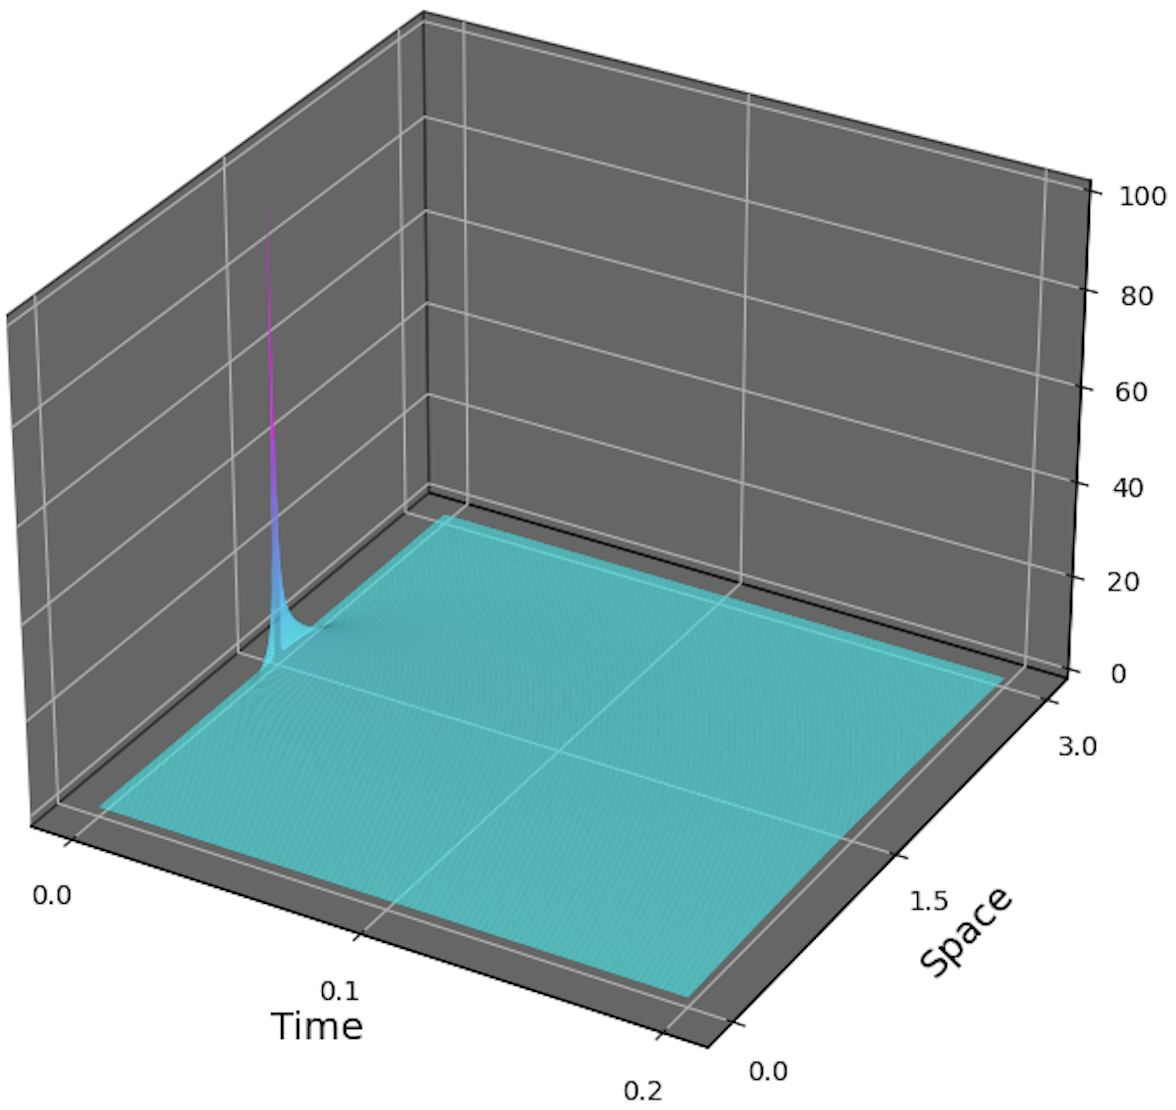
\includegraphics[width=\textwidth]{figs/deltaNoise0.png}
		\caption[]%
		{{\small $\lambda = 0$}}    
	\end{subfigure}
	\hfill
	\begin{subfigure}[b]{0.475\textwidth}  
		\centering 
		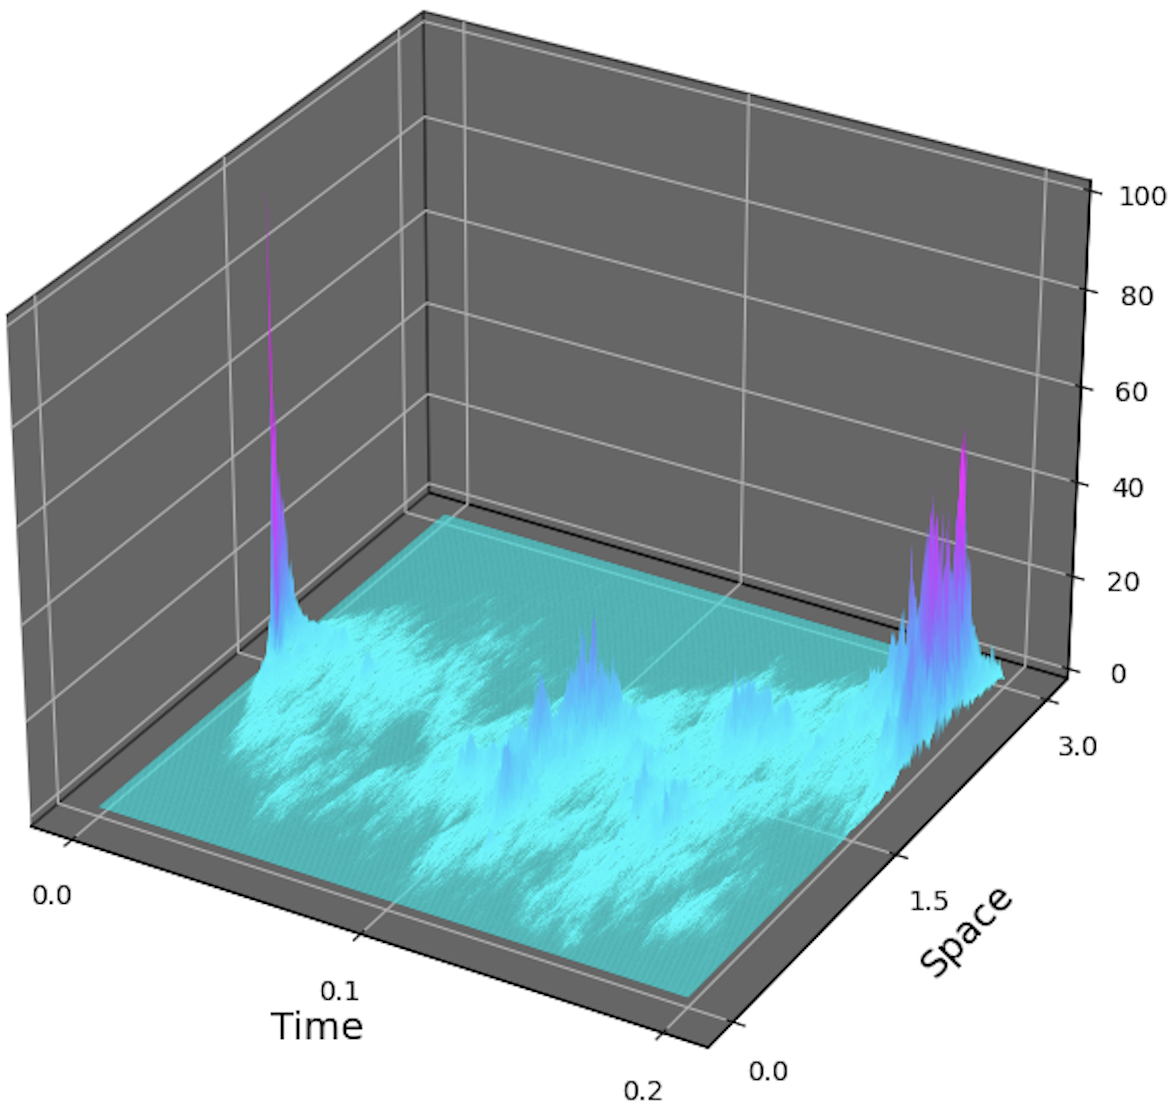
\includegraphics[width=\textwidth]{figs/deltaNoise1.8.png}
		\caption[]%
		{{\small $\lambda = 1.8$}}    
	\end{subfigure}
	\caption[] 
	{\small Simulations of Equation \eqref{E:introSHE} with $f(\cdot) = \delta_0(\cdot)$ and $\rho(u) = \lambda u$.} 
	\label{F:SHEsim1}
\end{figure*}

	\begin{theorem}
		Suppose that the function $\rho$ is globally Lipschitz function and the initial distribution $f(\cdot)$ satisfies the following:
			\[
				|\rho(x)| \le L_{\rho}^2(L_0^2 + |x|^2), \quad \text{and} \quad 	\int_{\R} \exp(-a|x|^2) \; f(\ud x) < \infty, 
			\]
		for some $L_b, L_0 > 0$ and any $a>0$. Then for $p \ge 2$, there exists a unique, $L^p(\Omega)$-continuous process that almost surely satisfies \eqref{E:introMsol}.
	\end{theorem}

\noindent It important to note that the above theorem allows for the initial condition to be the Dirac delta distribution. Moreover, this is a very natural choice and has many real world applications. 


\begin{figure*}
	\centering
	\begin{subfigure}[b]{0.475\textwidth}   
		\centering 
		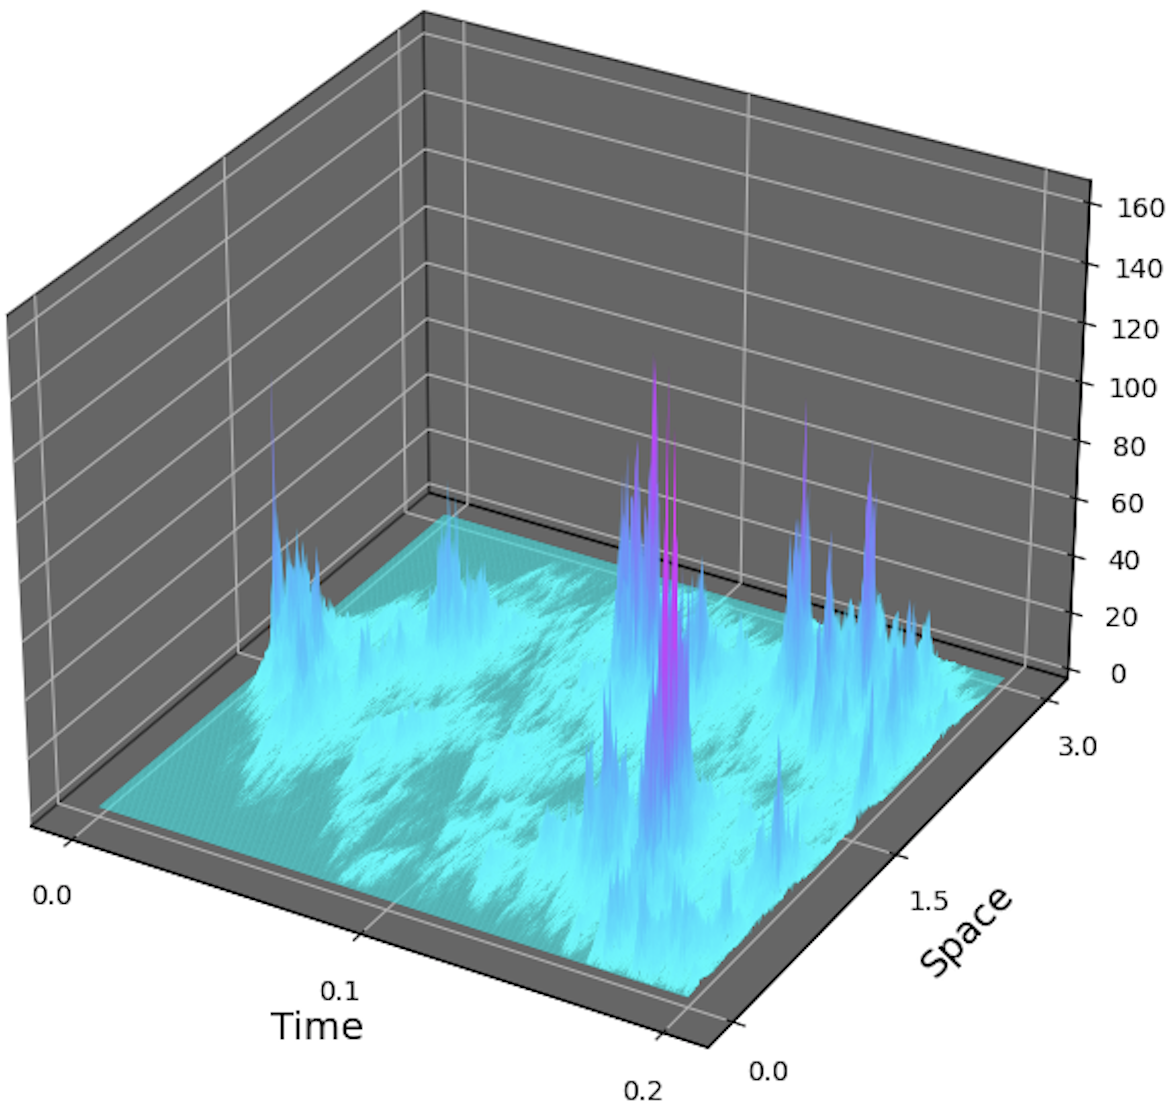
\includegraphics[width=\textwidth]{figs/deltaNoise2.2.png}
		\caption[]%
		{{\small $\lambda = 2.2$}} 
	\end{subfigure}
	\hfill
	\begin{subfigure}[b]{0.475\textwidth}   
		\centering 
		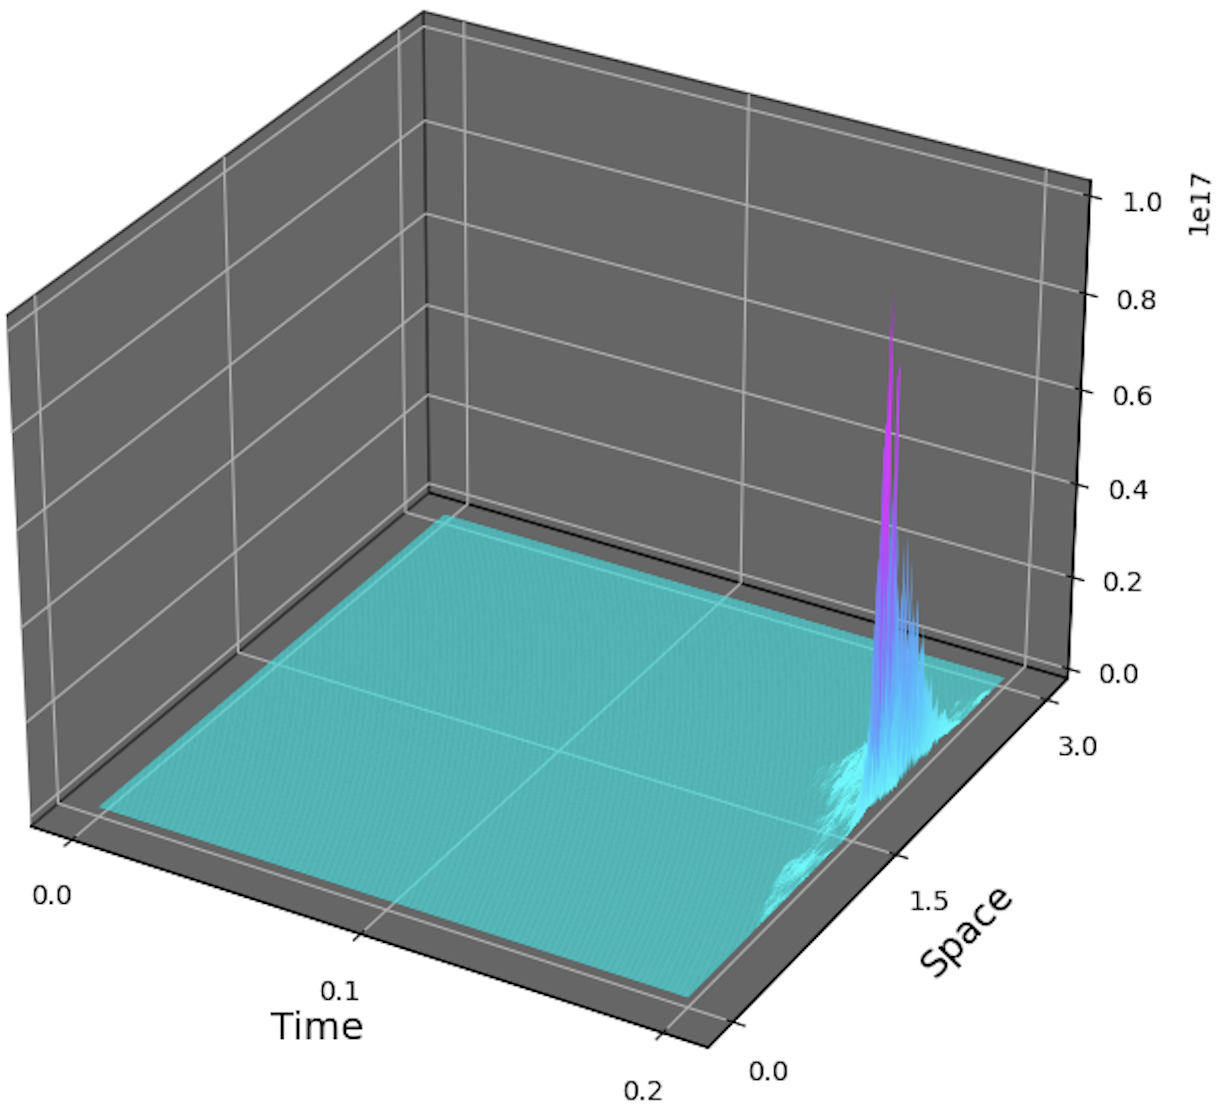
\includegraphics[width=\textwidth]{figs/deltaNoise2.8.png}
		\caption[]%
		{{\small $\lambda = 2.8$}}    
	\end{subfigure}
	\caption[] 
	{\small Simulations of Equation \eqref{E:introSHE} with $f(\cdot) = \delta_0(\cdot)$ and $\rho(u) = \lambda u$.} 
	\label{F:SHEsim2}
\end{figure*}

The simulations in Figures \ref{F:SHEsim1} and \ref{F:SHEsim2} illustrate a phenomena not seen in the deterministic case, that is, the formation of very large peaks widely separated by very deep valleys. This may seem unrealistic in practice but there is in fact a situation where one may make sense of this. Consider the $\delta_0(\cdot)$ initial condition to by representative of the "big bang" at the creation of our universe. One may assume that this is a highly random and chaotic event and that the transfer of heat may be roughly modeled Equation \eqref{E:introSHE} with $f(\cdot) = \delta_0(\cdot)$ and $\rho(u) = \lambda u$ for some "large" $\lambda > 0$. These tall, but isolated, peaks that form may be though of as the formation formation of galaxies and the empty space in between can just be thought of as the emptiness of outer space. Of course this is highly simplified, but still a nice way to picture what is happening in the simulations. 

Describing the growth of the peaks is an interesting question on its own. At the moment, it is an open question to describe the growth of the sample paths in time to the stochastic heat equation, in other words, the growth of the function
	\[
		t \mapsto u(t,x)(\omega), \quad x \in \R^d, \; \omega \in \Omega.
	\]
However, we do have some results on the growth in time of the $p^{th}$ moments of the solution for $p\ge2$. Some references that address this matter can found in \cite{chen.dalang:15:moments, chen.huang:19:comparison, chen.kim:19:nonlinear} and also Chapter \ref{C:ISHWEmom} below. Namely, in many cases of interest, the $p^{th}$ moments to the solution of the stochastic heat equation, and more generally the space-time fractional equation defined in Section \ref{S:ISHWE}, grow exponentially in time. This phenomena is reffered to as {\em intermittency}.

\section{Gaussian Noise}\label{S:Noise}
The driving force of a stochastic partial differential equation is the noise term, usually denoted by $\dot{W}$. Throughout this thesis we will considers three such types: white in time and white in space, white in time and colored in space, and time independent. We will now define each of the three. 


\subsection{White in time and either spatially white or colored} \label{SS:whitecolor}

We follow the set up as in \cite{dalang.khoshnevisan.ea:09:minicourse}. First, let $\Gamma(\ud x)$ be a non-negative and non-negative definite tempered measure, ie,
	\[
		\int_{\R^{d}} \Gamma(\ud x)(\phi * \tilde{\phi})(x) \ge 0, \quad \forall \; \phi \in \mathscr{L}(\R^d),
	\]
where $\mathscr{L}(\R^d)$ denotes the space of Schwartz functions and $\tilde{\phi}(x) = \phi(-x)$ and in addition 
	\[
		\int_{\R^d} \Gamma(\ud x) \; \frac{1}{(1 + |x|^2)^r} < \infty.
	\]
The Bochner-Schwartz theorem \cite{Schwartz.1966} guarantees the existence of a measure $\mu$, referred to as the {\em spectral measure}, whose Fourier transform is $\Gamma$: $\mathcal{F}\mu = \Gamma$. This means that 
	\[
		\int_{\R^d} \Gamma(\ud x) \phi(x) = \int_{\R^d} \mu(\ud \xi) \mathcal{F}\phi(\xi),
	\]
where we choose the following as our definition of the Fourier transform:
	\[
		\mathcal{F}\phi(\xi)  = \int_{\R^d} \ud x \; \exp\left(-i \xi \cdot x\right) \phi(x).
	\]

\begin{definition}
	Consider the $L^2(\Omega, \mathcal{F}, \mathbb{P})$ valued mean zero Gaussian process
		\[
			W = \left( W(\phi), \; \phi \in C_0^{\infty}(\R^{d+1}) \right)
		\]
	such that 
		\[
			\mathbb{E}\left(W(\phi)W(\psi)\right) = \int_0^\infty \ud s \int_{\R^{2d}} \Gamma(\ud x) \left( \phi(s,\cdot)*\tilde{\psi}(s ,\cdot) \right)(x).
		\]
	When $\Gamma(\ud x) = \delta_0(x)$ then $W$ is referred to as a {\em spatially homogeneous Gaussian space-time white noise}. Otherwise we say that $W$ is white in time and {\em colored} in space. 
\end{definition}

	   \begin{figure*}
	\centering
	\begin{subfigure}[b]{0.475\textwidth}
		\centering
		
\includegraphics[width=\textwidth]{figs/bsheet1.png}
%		\caption[]%
%		{}    
	\end{subfigure}
	\hfill
	\begin{subfigure}[b]{0.475\textwidth}  
		\centering 
		
\includegraphics[width=\textwidth]{figs/bsheet2.png}
%		\caption[]%
%		{}    
	\end{subfigure}
	\caption[] 
	{\small A simulation of two sample paths of a Brownian sheet.} 
	\label{F:bsheet}
\end{figure*}

\begin{proposition}[Proposition 4.19 \cite{da-prato.zabczyk:92:stochastic}] A space-time white noise is the distributional derivative of a Brownian sheet. See Figure \ref{F:bsheet}.
\end{proposition}

Note that in the case of a space-time white noise that the covariance takes the following form:
	\[
		\mathbb{E}\left(W(\phi)W(\psi)\right) = \int_0^\infty \ud s \int_{\R^{d}}\ud x \; \phi(s,x) \psi(s ,x),
	\]
and when the noise is colored and $\Gamma$ has density $f$ then the covariance takes the form
	\begin{equation} \label{E:CorrDensity}
		\mathbb{E}\left(W(\phi)W(\psi)\right) = \int_0^\infty \ud s \int_{\R^{2d}}\ud x \ud y \; \phi(s,x) f(x-y) \psi(s ,y).
	\end{equation}
Lastly, by the convolution property of the Fourier transform, we may say that 
	\[
		\mathbb{E}\left(W(\phi)W(\psi)\right) = \int_0^\infty \ud s \int_{\R^{d}} \mu(\ud \xi) \; \mathcal{F}\phi(s,\xi)  \overline{\mathcal{F}\psi(s , \xi)}.
	\]	
	
\begin{definition}
	Following \cite{walsh:86:introduction}, we extend $W$ to a sigma-finite $L^2(\Omega)$-valued measure $A \mapsto W(A)$ where is $A$ is a bounded Borel subset of $(0, \infty) \times \R^d$. We then define the {\em natural filtration}, $(\mathcal{F}_t)_{t \ge 0}$, where 
		\[
			\mathcal{F}_t = \sigma \left( W_s(A) : 0 \le s \le t, \; A \in \mathscr{B}_b((0,\infty) \times \R^d) \right) \vee \mathcal{N},
		\]
	where $\mathcal{N}$ denotes the set of $\mathbb{P}$-null sets in $\mathcal{F}$ and $\mathscr{B}_b((0,\infty) \times \R^d)$ is the space of bounded Borel subsets of $(0,\infty) \times \R^d$.
\end{definition}


\subsection{Time independent}\label{SS:timeind}

A time independent Gaussian noise is defined similarly as above.

\begin{definition}
	A {\em time-independent spatially homogeneous} Gaussian noise is a $L^2(\Omega, \mathcal{F}, \mathbb{P})$ valued mean zero Gaussian processes indexed on $C_0^{\infty}(\R^d)$,	
	\[
		W = \left(W(\phi) :  \phi \in C_0^{\infty}(\R^d)\right),
	\]
	with the following covariance structure
	\[
		\mathbb{E}\left(W(\phi)W(\psi)\right) = \int_{\R^{d}} \mu(\ud \xi)  \mathcal{F}\phi(\xi) \overline{\mathcal{F}\psi(\xi)},
	\]
	where we have the relation that $\Gamma = \mathcal{F}\mu$ just as we did in Section \ref{SS:whitecolor}.
\end{definition}


\section {The Stochastic Heat Equation} \label{S:SHE}
We will now introduce more formally the stochastic heat equation along with several important results that will be needed throughout this thesis. There many resources to choose for an introduction to the stochastic heat equation \cite{chen.dalang:15:moments, chen.kim:19:nonlinear, dalang.khoshnevisan.ea:09:minicourse, da-prato.zabczyk:92:stochastic, khoshnevisan.cbms.2014, walsh:86:introduction}. 

Recall from \eqref{E:introSHE} that the stochastic heat equation can be written informally in the following way:
	
	\begin{equation}\label{E:SHE}
\begin{cases}
\frac{\partial u}{\partial t}(t,x)  = \frac{\nu}{2} \Delta_xu(t,x) + \rho(u(t,x))\dot{W}(t,x) & t \ge 0, \; x \in \R^d \\
u(0,x) = \mu(\cdot) & x \in \R^d.
\end{cases}
\end{equation}
The initial distribution $\mu$ is a deterministic and locally finite Borel measure which must satisfy the following inequality 
	\begin{equation}\label{A:InitCon}
		\int_{\R^d} \exp\left(-a |x|^2\right) |\mu|(\ud x) < \infty, \quad \text{for all } a > 0,
	\end{equation}
where $|\mu| = \mu^+ + \mu^-$. In general, $d \ge 1$, $\nu >0$ and the noise may be either of the three noises introduced in Section \ref{S:Noise}. However, as we will see in Chapter \ref{C:InvMeas}, our only case of interest is when $d \ge 3$ and the noise is white in time and colored in space. For that reason we will restrict ourselves to that case.

We will denote by $\hat{f}(\ud \xi)$, the spectral measure of the noise $\dot{W}$ and in the case when $\Gamma$ has density $f$, as in \eqref{E:CorrDensity} above, then the spectral measure takes the form $\hat{f}(\xi) \ud \xi$. We define the following property known as {\em Dalang's condition}:
	\begin{equation}\label{A:DalCon}
		\Upsilon(\beta) := \int_{\R^d} \frac{\hat{f}(\ud \xi)}{\beta + |\xi|^2} < \infty, \quad \text{for some and hence all } \beta > 0.
	\end{equation}
By a solution to \eqref{E:SHE}, we mean a solution to the following stochastic integral equation:
	\begin{align}
		u(t,x) &= \int_{0}^\infty G(t,x-y) \mu (\ud y) + \int_0^t\int_{\R^d} G(t-s, x-y) \rho(u(s,y)) W(\ud s, \ud y) \nonumber \\
		&= J_0(t,x) + I(t,x) \label{E:MildSolSHE}
	\end{align}
where the above is a {\em Walsh} stochastic integral \cite{walsh:86:introduction} and $G$ is the heat kernel 
	\[
		G(t,x) = (2\pi \nu t)^{-d/2} \exp\left(-\frac{|x|^2}{2 2 \nu t}\right).
	\]
\begin{definition}
	A random field $u = (u(t,x) : t \ge 0, \; x \in \R^d)$ is a {\em mild solution} to \eqref{E:SHE} if 
		\begin{enumerate}
			\item $u$ is adapted to the filtration generated by the noise $W$,
			\item $u$ is jointly measureable with respect to $\mathscr{B}((0,\infty) \times \R^d) \times \mathcal{F}$,
			\item $\Norm{I(t,x)}_2 < \infty$ for all $(t,x) \in (0,\infty) \times \R^d$,
			\item $u$ satisfies \eqref{E:MildSolSHE} a.s. for all $(t,x) \in (0,\infty) \times \R^d$.
		\end{enumerate}
\end{definition}

We have the following solvability theorem 

\begin{theorem}[Theorem 2.4 \cite{chen.kim:19:nonlinear}] \label{T:SHEsolve}
	Suppose that the initial distribution and the spectral measure satisfy both \eqref{A:InitCon} and \eqref{A:InitCon} respectively. Suppose that $\rho$ is globally Lipschitz with Lipschitz constant $L_rho$. Then there exists a unique (in the sense of versions) random-field solution starting from $\mu$ that is $L^2(\Omega)$-continuous. 
\end{theorem}

The next result gives us a very useful bound on the $p^{th}$ moments of the solution. In order to fully utilize the result, we need to strengthen some of our assumption to the following:
	\begin{equation} \label{E:U0finite}
	\Upsilon(0) := \int_{\R^d} \frac{\hat{f}(\ud \xi)}{|\xi|^2} <\infty \quad \text{and} \quad
	64L^2_{b}   <  \frac{1}{4\Upsilon(0)};
	\end{equation}

%\begin{theorem}[Theorem 1.7 \cite{chen.huang:19:comparison}]
%	Under the same assumptions of Theorem \ref{T:SHEsolve}, for any $p \ge 2$, $t > 0$ and $x \in \R^d$ we have that 
%		\[
%			\Norm{u(t,x)}_p \le C \left[\bar\varsigma + \sqrt{2}(G(t,\cdot)*|\mu|)(x)\right]H(t; \gamma_p)^{1/2}
%		\]
%	where $\bar\varsigma = |\rho(0)|/L_\rho$, $\gamma_p = 32pL_\rho^2$ and $H(t;\gamma_p)$ is a nondecreasing function in $t$ whose exact definition is not important in this setting. Moreover, under the added assumption that  
%\end{theorem}

\begin{theorem}[Theorem 1.7 \cite{chen.huang:19:comparison}, Lemma 2.5 \cite{chen.kim:19:nonlinear}] \label{T:ExUn}
	Under the assumptions of Theorem \ref{T:SHEsolve}, for any $t>0$ and $x \in \R^d$, the solution to
	\eqref{E:SHE}, $u(t,x)$, is in $L^p(\Omega)$ and for $p\ge 2$
	\begin{equation} \label{E:mb}
	\Norm{u(t,x)}_p \le \big[\bar{\varsigma}+\sqrt{2}(G(t,\cdot) * |\mu|)(x)\big]H(t;\gamma_p)^{1/2},
	\end{equation}
	where $\bar{\varsigma}=|\rho(0)|/L_{\rho}$, $\gamma_p = 32pL_{\rho}^2$ and the function $H(t;\gamma_p)$ is nondecreasing in $t$ (see \cite{chen.huang:19:comparison} for the expression of $H$). Moreover, if two conditions in \eqref{E:U0finite} hold,
	% \begin{equation}\label{A:dalcon0}
	%   \Upsilon(0) < \infty \quad \text{and} \quad \gamma_p < \frac{1}{4\Upsilon(0)},
	% \end{equation}
	then this function $H(t;\gamma_p)$ is bounded in $t$. Hence, by choosing $C=\left(\sqrt{2}\vee
	\overline{\varsigma}\right)\sup_{t\ge 0} H(t;\gamma_p)^{1/2}<\infty$, we have that
	\begin{equation} 
	\Norm{u(t,x)}_p \le C\bigg(1+ (G(t, \cdot)*|\mu|)(x) \bigg).
	\end{equation}
\end{theorem}


\section { \normalfont The Interpolated Stochastic Heat and Wave Equation} \label{S:ISHWE}

We will consider the ISHWE driven by all three noises introduced in Section \ref{S:Noise}. The set up for the time-independent case is much different so we will address that case separately in Section \ref{SS:ISHWEtimeind}. We will then introduce the set with either a space-time white noise or a noise that is white in time and colored in space in Section \ref{SS:ISHWEnoisetime}.

Before stating the equation, we need to define some fractional differential operators. We start with the {\em fractional Laplacian}. Recall the formula
	\[
	(-\Delta) f (x) = ((|\cdot|^{2})\hat{f}(\cdot))^{\vee}(x).
	\]
Following \cite{grafakos:14:modern}, we are then motivated to define the fractional Laplacian of order $0 < \alpha < d$ as
	\begin{equation} \label{D:fraclaplacian}
		(-\Delta)^{\alpha / 2} f (x) := ((|\cdot|^{\alpha})\hat{f}(\cdot))^{\vee}(x),
	\end{equation}
where $\widehat f$ and $\widecheck f$ are shorthand for the Fourier and inverse Fourier transform of $f$ respectively. Thus, the fractional Laplacian can be written as a convolution,
	\[
			(-\Delta)^{\alpha / 2} f (x) = ( (R_{d-\alpha}(\cdot) * f(\cdot)) (x),
	\]
where (see \cite[Example 1.3]{balan.chen.chen:03:invariant})
	\begin{align*}
		R_{d-\alpha}(x) &= (2\pi)^{-d} (|\cdot|^\alpha)^{\vee}(x) \\
		& = 2^{-\alpha} \frac{(2\pi)^{-d}}{\pi^{d/4}} \frac{\Gamma((d-\alpha)/2)}{\Gamma(\alpha/2)}|x|^{-d+\alpha}.
	\end{align*}
Next we define the {\em Caputo derivative} of order $\beta > 0$ as 
	\[ \partial^{\beta}f(t) :=
		\begin{cases}
			\frac{1}{\Gamma(m- \beta)} \int_0^t \ud \tau \; \frac{f^{(m)}(\tau) }{(t-\tau)^{\beta + 1 -m}} & m-1 < \beta < m \\
			\frac{d^m}{dt^m}f(t) & \beta = m.
		\end{cases}
	\]
Lastly we define the {\em Riemann-Liouville fractional integral} of order $\gamma > 0$ as 
	\[
		I_t^{\gamma} f(t) := \frac{1}{\Gamma(\gamma)} \int_0^t (t-s)^{\gamma -1} f(s) \ud s.
	\]
For more on $\partial^{\beta}$ and $I_t^{\gamma}$ see \cite{podlubny.1999}.

\subsection{Time-independent noise case} \label{SS:ISHWEtimeind}

The {\em interpolated stochastic heat equation} (ISHWE) driven by a time-independent Gaussian noise is given by 
	\begin{equation} \label{E:ISHWE}
	\begin{cases}
	\left(\partial^b_t + \frac{\nu}{2}(-\Delta)^{a/2}\right)\: u(t,x) = I^r_t \left[\sqrt{\theta}\: u(t,x)\: \dot W(x) \right] & \text{$x\in \R^d$, $t>0$}, \\
	u(0,\cdot) = 1                                                                                                             & b \in (0,1],               \\
	u(0,\cdot) = 1, \quad \partial_t u(0,\cdot) = 0                                                                            & b \in (1,2),
	\end{cases},
	\end{equation}
where $a \in (0,2)$, $b \in (0,2)$, $r\ge0$, $\nu >0$ and $\theta > 0$. We recall from above that 
	\[
		\mathbb{E}[W(\phi)W(\psi)] = \int_{\R^d} \mathcal{F}\phi(\xi) \overline{\mathcal{F}\psi(\xi)} \mu(\ud \xi) =: \mathcal{H},
	\]
where $\mu$ is the spectral measure of the noise.

The
fundamental solution to \eqref{E:ISHWE} is expressed explicitly in terms of the {\it Fox H-function},
$H^{m,n}_{p,q}(z)$, which is much more complicated than the Green's function for either the heat or
wave equation. In this case, we denote the fundamental solution as
\begin{equation} \label{E:GreenFunction}
G(t,x):= G_{a,b,r,\nu,d}(t,x),
\end{equation}
where
\[
G_{a,b,r,\nu,d}(t,x) = \pi^{-d/2} |x|^{-d} t^{b+r-1} H^{2,1}_{2,3}\left( \frac{|x|^a}{2^{a-1}\nu t^b}\;  \Bigg \vert  \begin{array}{l}
(1,1),\; (b+r,b) \\
(d/2,a/2),\; (1,1),\; (1,a/2)
\end{array} \right).
\]
We direct the reader to Theorem 4.1\footnote{$G(t,x)$ corresponds to $Y_{a,b,r,\nu,d}(t,x)$ from
	\cite{chen.hu.nualart:19:spacetimefrac}.} of \cite{chen.hu.nualart:19:spacetimefrac} for more details. Since we are interested in the constant one initial
condition (and zero initial velocity when $b>1$), Theorem 4.1 ({\it ibid.}) implies that the
corresponding solution to the homogeneous equation (i.e. the solution when there is no driving
source) is equal to the constant one. Hence through superposition, \eqref{E:ISHWE} can be written as
the following stochastic integral equation:
\begin{equation} \label{E:spdeint}
u(t,x) = 1 + \sqrt{\theta}\int_0^t \left( \int_{\R^d}G(t-s,x-y)u(s,y) W(\delta y) \right) \ud s,
\end{equation}
where the stochastic integral is in the {\it Skorohod} sense (see \cite{nualart.nualart:18:malliavin}). The reason for choosing to define the solution through the Skorohod integral is due the the fact that the noise is no longer white in time. Because if this, we may no longer use the theory of Walsh \cite{walsh:86:introduction}.

	   \begin{figure*}
	\centering
	\begin{subfigure}[b]{0.32\textwidth}
		\centering
		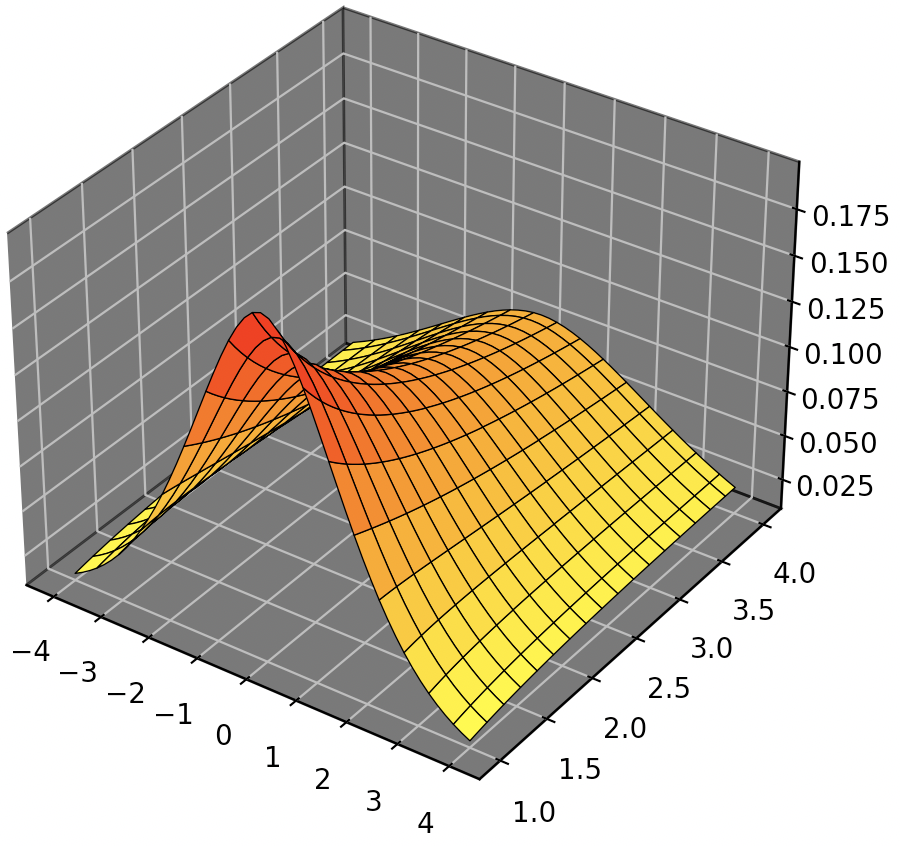
\includegraphics[width=\textwidth]{figs/Yb.7.png}
				\caption[]%
				{b = .7}    
	\end{subfigure}
	\hfill
	\begin{subfigure}[b]{0.32\textwidth}
		\centering
		
\includegraphics[width=\textwidth]{figs/Yb1.png}
		\caption[]%
		{b = 1}    
	\end{subfigure}
	\hfill
	\begin{subfigure}[b]{0.32\textwidth}  
		\centering 
		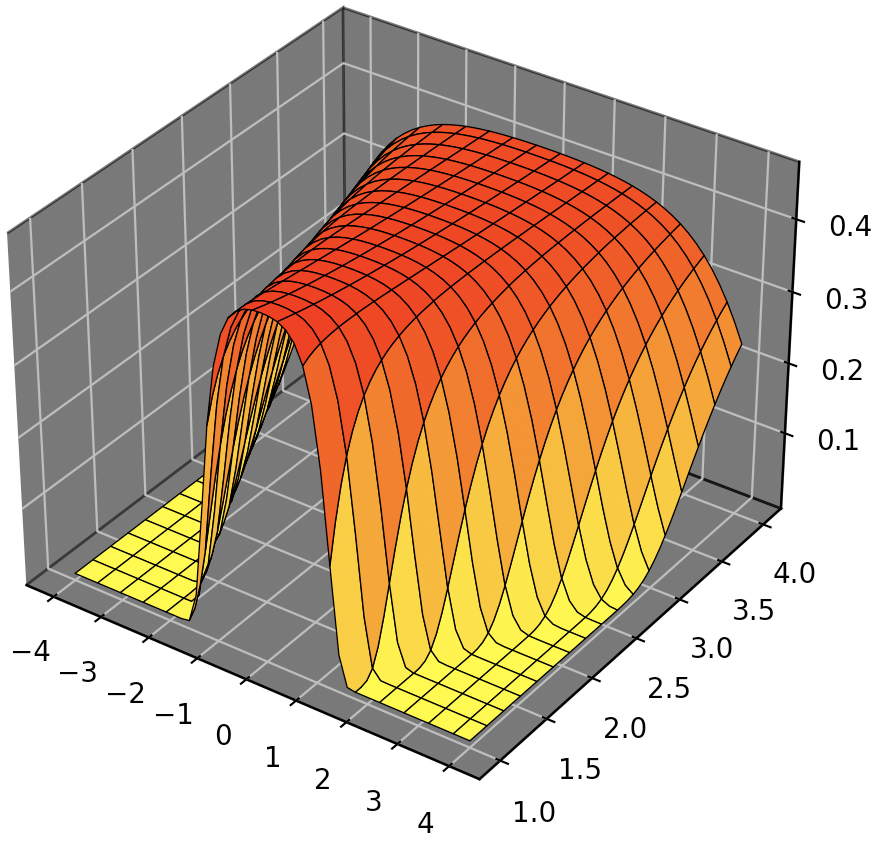
\includegraphics[width=\textwidth]{figs/Yb1.8.png}
				\caption[]%
				{b = 1.8}    
	\end{subfigure}
	\caption[] 
	{\small Some plots of $G_{2,b,0,2,1}(t,x)$ with $-4 \le x \le 4$ and $1 \le t \le 4$.} 
\end{figure*}

We now formalize this in the next definition.

\begin{definition}[Mild, local and global solutions] \label{D:Sol}
	(1) For $T\in (0,\infty]$, a random field $u=\left\{u(t,x) : t \in (0,T),\: x\in\R^d\right\}$ is
	called {\it a mild solution} to the equation \eqref{E:ISHWE} if for all $x\in\R^d$ and $s,t$ fixed
	with $0<s\le t <T$, $y\to G(t-s,x-y)u(s,y)$ is Skorohod integrable and the following stochastic
	integral equation holds almost surely
	\begin{equation} \label{E:ISHWEIntEq}
	u(t,x) = 1 + \sqrt{\theta}\int_0^t \left( \int_{\R^d} G(t-s,x-y)u(s,y) W(\delta y) \right)\ud s.
	\end{equation}
	
	\noindent (2) Let $u(t,x)$ be a mild solution to \eqref{E:ISHWE} (or \eqref{E:ISHWEIntEq}) and fix $p\ge
	1$. We call $u(t,x)$ a {\it global $L^p(\Omega)$-solution}, or simply an {\it
		$L^p(\Omega)$-solution} if
	\begin{align} \label{E:Lp}
	\Norm{u(t,x)}_p < \infty \qquad \text{for all $t>0$ and $x \in \R^d$.}
	\end{align}
	
	\noindent (3) If there exist $0<T_1\le T_2<\infty$ such that $\Norm{u(t,x)}_p$ is finite for all
	$t\in(0,T_1)$ and $x\in\R^d$, but $\Norm{u(t,x)}_p$ diverges to infinity whenever $t>T_2$, the mild
	solution $u(t,x)$ in this case is called a {\it local $L^p(\Omega)$-solution}.
\end{definition}

The existence and uniqueness of the solution will be proven in Chapter \ref{C:ISHWEmom}. We now finish this section with some more preliminary facts that will be needed later on. Note that through construction of the Skorohod integral $\delta$, a mild solution is necessarily to
be an $L^2(\Omega)$-solution.  For more details, one may check, e.g., Nualart \cite[Chapter
3]{nualart.nualart:18:malliavin}.  \bigskip

Through the standard {\it Picard iteration} scheme, the solution can be expressed by the following
{\it Wiener chaos expansion} \footnote{Wiener chaos expansion has been widely to solve the linear
	stochastic partial differential equations. We direct interested readers to \cite[Section
	5]{balan.song:17:wavespacetimecolor} for a presentation of this procedure.}:
\begin{equation} \label{E:solwexp}
u(t,x) = 1 + \sum_{k=1}^\infty \theta^{k/2}I_k(f_k(\cdot,x,t)),
\end{equation}
where $I_k : \mathcal{H}^{\otimes k}\left((\R^d)^k\right) \to \mathcal{H}_k$ is the $k^{th}$ order
Skorohod integral and $\mathcal{H}_k$ is the $k^{th}$ Wiener chaos space and the kernels
$f_k(\cdot,x,t)$, obtained through the iteration, are equal to
\begin{align*}
% \label{E:wker}
f_n(x_1,...,x_k;x,t)
& = \int_0^t \int_0^{t_n}\cdots \int_0^{t_2} G(t-t_n,x-x_n)\cdots G(t_2-t_1,x_2-x_1) \ud t_1\cdots \ud t_n \\
& = \int_0^t \int_0^{t_n}\cdots \int_0^{t_2} G(t_1,x-x_n)\cdots G(t_n-t_{n-1},x_2-x_1) \ud t_1\cdots \ud t_n. \nonumber
\end{align*}
For ease of notation, throughout this article, we may write the above integrals as
\begin{align*}
f_n(x_1,...,x_n;x,t)
& = \int_{[0,t]^n_<} G(t-t_n,x-x_n)\cdots G(t_2-t_1,x_2-x_1) \ud \vec{t} \\
& = \int_{[0,t]^n_<}G(t_1,x-x_n)\cdots G(t_n-t_{n-1},x_2-x_1) \ud \vec{t},
\end{align*}
where $[0,t]_<^n:=\{(t_1,\cdots,t_n)\in [0,t]^n:\: t_1<\cdots < t_n\}$ and $\ud \vec{t} = \ud t_1 \cdots \ud t_n$. As usual, we use
$\widetilde{f_n}(\cdot, x, t)$ to denote the symmetrization of $f_n(\cdot,x,t)$:
\begin{align*}
\widetilde{f_n}(\cdot; x, t)
& = \frac{1}{n!} \sum_{\rho \in \Sigma_n} f_n\left(x_{\rho(1)},\cdots, x_{\rho(n)}\right) \\
& = \frac{1}{n!} \sum_{\rho \in \Sigma_n} \int_{[0,t]^n_<} G\left(t-t_n,x-x_{\rho(n)}\right)\cdots G\left(t_2-t_1,x_{\rho(2)}-x_{\rho(1)}\right) \ud \vec{t},
\end{align*}
where $\Sigma_n$ is the set of all permutations of $\{1,\cdots,n\} $.
% In particular, for $x=0$ we have
% \begin{align}
%   \label{E:fperm0}
%   \widetilde{f_n}(\cdot; 0, t) = \frac{1}{n!} \sum_{\rho \in \Sigma_n} \int_{[0,t]^n_<} G(t_1,x_{\rho(1)})\cdots G(t_n-t_{n-1},x_{\rho(n)}-x_{\rho(n-1)}) \ud \vec{t}.
% \end{align}
By setting $t_{n+1}=t$, the Fourier transform of the kernels, $f_n$, is given by
\begin{align} \label{E:fweker}
\mathcal{F}f_n(\cdot;x,t)(\xi_1,...,\xi_n)
= e^{-i \left(\sum_{j=1}^n \xi_j \right) \cdot x} \int_{[0,t]^n_<}
\prod_{k=1}^n \overline{\mathcal{F}G(t_{k+1}-t_k,\cdot)\left(\sum_{j=1}^k \xi_j\right) } \ud \vec{t}.
\end{align}

Recall the notation above in \eqref{E:GreenFunction} that $G(t,x) = G_{a,b,r,d}(t,x)$. The following
scaling properties for both $\mathcal{F}G(t,\cdot)(\xi)$ and
$\Norm{\widetilde{f_n}(\cdot,x,t)}_{\mathcal{H}^{\otimes n}}$ play an important role in the paper.

\begin{lemma} \label{L:Scale}
	For any $c,t>0$, $n\ge 1$, $\xi,\xi_1,\cdots,\xi_n\in\R^d$, the following scaling properties hold:
	\begin{gather} \label{E:greenscale}
	\mathcal{F}G(t,\cdot)(c\xi) = c^{-\frac{a}{b}(b+r
		-1)}\mathcal{F}G\left(c^{\frac{a}{b}}t,\cdot\right)( \xi) \quad \text{and} \quad
	\mathcal{F}G(ct,\cdot)(\xi) = c^{b+r -1}\mathcal{F}G(t,\cdot)(c^{b/a} \xi), \\
	\label{E:Ffnscale} \mathcal{F}\widetilde{f}_n(\cdot,0,ct)(\xi_1,\cdots,\xi_n) = c^{n(b+r)}
	\mathcal{F}\widetilde{f}_n(\cdot,0,t)(c^{b/a}\xi_1, \cdots, c^{b/a}\xi_n), \\
	\label{E:normscale} \Norm{\widetilde{f_n}(\cdot,0,t)}_{\mathcal{H}^{\otimes n}}^2 = t^{[2(b + r
		) -b \alpha / a]n} \Norm{\widetilde{f_n}(\cdot,0,1)}_{\mathcal{H}^{\otimes n}}^2.
	\end{gather}
\end{lemma}
\begin{proof}
	The scaling properties in \eqref{E:greenscale} are direct consequences of the explicit expression
	of $\mathcal{F}G(t,\cdot)(\xi)$ as in \cite[(4.8)]{chen.hu.nualart:19:spacetimefrac}. Property \eqref{E:Ffnscale} is an easy
	exercise of change of variables on \eqref{E:fweker}. Property \eqref{E:normscale} is a direct
	consequence of \eqref{E:greenscale}, \eqref{E:Ffnscale}, and the scaling property of the spectral
	measure $\mu$. We leave the details for the interested readers.
\end{proof}

Finally, let us recall the following standard result about the existence and uniqueness of the
solution to \eqref{E:ISHWE} (or \eqref{E:ISHWEIntEq}) when it can be written as the Wiener chaos expansion
\eqref{E:solwexp}.

\begin{theorem}\label{T:2momseries}
	Fix any $T \in (0,\infty]$. Suppose that $f_n(\cdot,x,t) \in \mathcal{H}^{\otimes n}$ for any $t
	\in (0,T)$, $x \in \R^d$ and $n \ge 1$. Then \eqref{E:ISHWE} (or \eqref{E:ISHWEIntEq}) has a unique
	$L^2(\Omega)$-solution on $(0,T) \times \R^d$ if and only if the series \eqref{E:solwexp}
	converges in $L^2(\Omega)$ for any $(t,x) \in (0,T) \times \R^d$, which is equivalent to the
	convergence of the series \eqref{E:2mom}. In this case, the solution is given by \eqref{E:solwexp}
	with the second moment given by
	\begin{equation} \label{E:2mom}
	\mathbb{E}\left(u(t,x)^2\right)
	= \sum_{n \ge 0} \theta^n n!  \Norm{\widetilde{f_n}(\cdot,x,t)}_{\mathcal{H}^{\otimes n}}^2
	\quad \text{for all $(t,x) \in (0,T) \times \R^d$}.
	\end{equation}
\end{theorem}



\subsection{Time-dependent noise case} \label{SS:ISHWEnoisetime}
Will fill out if the project is completed in time.


\chapter{ \normalfont Invariant Measures for the Stochastic Heat Equation} \label{C:InvMeas}

text...

\chapter{ \normalfont Exact Moment Asymptotics for the Interpolated Stochastic Heat and Wave Equation} \label{C:ISHWEmom}

text...


\chapter{ \normalfont Existence of Global Solutions to the ISHWE with a Super-linear Diffusion Term}\label{C:Global}

text...








%%%%%%%%Two options for having a bibliography. If you use a separate file or multiple files:
%\bibliography{./robotics,./imageprocessing,./thesis}
%%%%% where the files are robotics.bib, imageprocessing.bib and/or thesis.bib. 

%Or you can include the bibliography entries directly:

%\begin{thebibliography}{99}
%%\newcommand{\AmS}{$${\protect\the\textfont2 A}\kern-.1667em\lower
%%         .5ex\hbox{\protect\the\textfont2 M}\kern
%%         -.125em{\protect\the\textfont2 S}}
%
%\bibitem{hahn} Jane Hahn, ``\LaTeX{} For Everyone,'' Personal TeX Inc., 
%  12 Madrona Street, Mill Valley, California.
%
%\end{thebibliography}

% {{{ All references: New ones with biber
\addcontentsline{toc}{section}{References}
\printbibliography[title={References}]
% }}}



\appendix
\chapter*{Appendices\addcontentsline{toc}{chapter}{Appendices}}

\chapter{Notes on the style-file project}

\begin{singlespace}
These style-files have been modified by Christopher Wilson to support the new Electronic Thesis and Dissertation process. The following was written before the ETD guidelines update on Fall 2009. Changes to the original appendix have been shown in italics. 

These style-files for use with \LaTeX{} {\it were} maintained by Darrel
Hankerson\footnote{Mathematics and Statistics, 221 Parker Hall,
844-3641, {\tt hankedr@auburn.edu}} and Ed
Slaminka\footnote{Mathematics and Statistics, 218 Parker,
{\tt slamiee@auburn.edu}}.

In 1990, department heads and other representatives met with Dean Doorenbos
and Judy Bush-Crofton (then responsible for manuscript approval). This
meeting was prompted by a memorandum\footnote{Originally, the memorandum
was presented to Professor Larry Wit. A copy is available on request.} from
members of the mathematics departments concerning the {\em Thesis and
Dissertation Guide\/} and the approval process. There was wide agreement
among the participants (including Dean Doorenbos) to support the basic
recommendations outlined in the memorandum. The revised {\em Guide\/}
reflected some (but not all) of the agreements of the meeting.

Ms Bush-Crofton was supportive of the plan to obtain ``official approval''
of these style files.\footnote{Followup memoranda gave a definition of
``official approval.'' Copies will be sent on request.}  Unfortunately, Ms
Bush-Crofton left the Graduate School before the process was completed. In
1994, we were revisiting some of the same problems which were
resolved at the 1990 meeting.

In Summer 1994, I sent several memoranda to Ms Ilga Trend of the Graduate
School, reminding her of the agreements made at the 1990 meeting.
Professors A. Scottedward Hodel and Stan Reeves provided additional
support.  In short, it is essential that the Graduate School honor its
commitments of the 1990 meeting. It should be emphasized that Dean
Doorenbos is to thank for the success of that meeting.

Maintaining these \LaTeX{} files has been more work than expected, in
part due to continuing changes in requirement by the graduate school.
The Graduate School occasionally has complete memory loss about the
agreements of the 1990 meeting. If the Graduate School rejects your
manuscript based on items controlled by the style-files, ask
your advisor to contact the Graduate school (and copy to me) to urge
cooperation.

Finally, there have been several requests for additions to the package
(mostly formatting changes for figures, etc.). While such changes are not
really part of the thesis-style package, it could be beneficial to collect
these options and distribute with the package (making it easier on the next
student).  I'm especially interested in changes needed by various
departments.

\end{singlespace}

\end{document}

